\begin{figure}[bth!]
	\begin{center}
		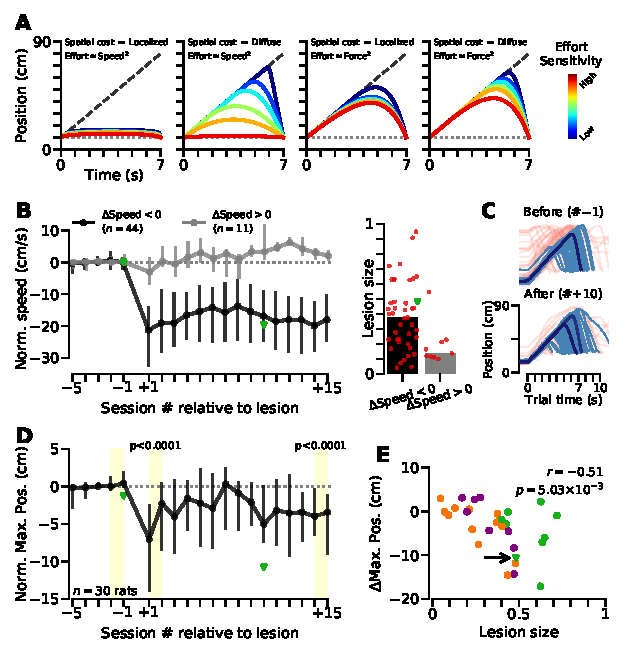
\includegraphics[scale=1]{ch-lesion/figures/MaxPosAnalysis.pdf}
		\caption[Optimal Trajectory and Experimental Validation]
		{\textbf{Optimal trajectory vs.\ effort sensitivity and experimental validation.}
		\textbf{A)}
		Optimal trajectories predicted by models with different effort and spatial costs approximations.
		The cost of premature entrance in the reward area (spatial cost) was simulated using a Heaviside function that was either localized ($\sim$step function with non-zero value within the reward area) or diffuse ($\sim$a sigmoid function whose value gradually decreases toward zero away from the reward area).
		Effort was approximated as the square value of either the modeled muscular force produced by the animals or of its speed.
		\textbf{B)}
		\textit{Left}: animals were divided into two groups based on the impact of the striatal lesion on their running speed.
		\textit{Right}: lesion size for animals in those two groups.
		Green triangles in panels~B,~D, and~E are data points from the example animal whose trajectories, before and after lesion, are shown in panel~C.
		\textbf{C)}
		Effect of striatal lesion on the trajectories of a single animal.
		Only trials in which the routine was executed (thin blue lines) were taken into account to find the trajectory of median maximum position (tick blue line).
		The shadow of the trajectory of median maximum position before lesion is displayed in the bottom plot for comparison.
		\textbf{D)}
		Effect of striatal lesion on the median maximum position in routine trials.
		\textbf{E)}
		Effect of striatal lesion on the median maximum position vs.\ lesion size.
		Same color code for individual lesion type as in \autoref{fig:lesion:task}.
		}
		\label{fig:lesion:maxPos}
	\end{center}
\end{figure}